\documentclass[hyperref={pdfpagelabels=false}]{beamer}
\usepackage{CJKutf8}
\usepackage[english]{babel}
\usepackage{xcolor}
\usepackage{lmodern}
\usepackage{amssymb}
\usepackage[makeroom]{cancel} %for crossing symbols
\usepackage{leftindex} %For leftindex, making it possible to have nicely aligned left subscripts
%\usepackage{calligra}
%\DeclareMathAlphabet{\mathcalligra}{T1}{calligra}{m}{n} %For small \mathcal letters
\makeatletter
\DeclareFontEncoding{LS1}{}{}
\DeclareFontSubstitution{LS1}{stix}{m}{n}
\DeclareMathAlphabet{\mathKel}{LS1}{stixscr}{m}{n}
\DeclareMathAlphabet{\mathcal}{LS1}{stixscr}{m}{n}
\usepackage{amsthm}
\usepackage{amsmath}
%\usepackage{mathabx}
\usepackage{stmaryrd}
\usepackage{amsbsy}
\usepackage{dsfont}
\usepackage{mathtools} %für mathclap und coloneqq
%\usepackage{amsbsy}
\usepackage{mleftright} %Distanz zu \left \right weg
\usepackage{tikz-cd}

\usepackage{tabularx} %Automatic line break of tables using X instead c l r
%\usepackage{longtable} %table auf mehreren Seiten
%\usepackage{ltxtable} %Combination of both above
\usepackage{xcolor, colortbl}

%Für die ganzen Diagramme
\usepackage{pgfplots}
\usepackage{graphicx} %Für raisebox, vertical displacement of figures
\usetikzlibrary{decorations.markings, decorations.text,calc,arrows.meta}

\definecolor{Gray}{gray}{0.85}
%\usepackage[style=authortitle-icomp]{biblatex}
%\usepackage[babel,german=guillemets]{csquotes}

\setcounter{tocdepth}{1}
%\setcounter{tocdepth}{5}
%\setcounter{secnumdepth}{4}
%\setcounter{secnumdepth}{5}
\usepackage[backend=biber, style=numeric]{biblatex}
\addbibresource{Literatur.bib}
\newcommand{\footlineextra}[1]{
    \begin{tikzpicture}[remember picture,overlay]
        \node[yshift=2ex,anchor=south west] at (current page.south west) {\usebeamerfont{author in head/foot}\hspace{2ex}#1};
    \end{tikzpicture}
}

\newcommand\insertreferences{}
\setbeamertemplate{footline}{%
  \leavevmode%
  \hbox{%
  \begin{beamercolorbox}[wd=.09\paperwidth, ht=5ex,dp=1ex,center, sep=1.4ex]{author in head/foot}%
    \usebeamerfont{author in head/foot}
		%\vfill
		%Sources
		%\vfill
		Sources
  \end{beamercolorbox}%
  \begin{beamercolorbox}[wd=.91\paperwidth,ht=5ex,dp=1ex,center]{title in head/foot}%
    \usebeamerfont{title in head/foot}
    \insertreferences

  \end{beamercolorbox}
}
}


%%% Transition slides
\AtBeginSection[]{
  \begin{frame}
  %\vfill
	\thispagestyle{empty}
  \centering
  \begin{beamercolorbox}[sep=8pt,center,shadow=true,rounded=true]{title}
    \usebeamerfont{title}\insertsection\par%
  \end{beamercolorbox}
  %\vfill
  \end{frame}
}

\title{Curved gauge theories and their applications}   
\subtitle{}   
\author{Simon-Raphael Fischer} 
\institute{
\begin{figure}
	\centering
		
\includegraphics[width=.50\textwidth]{NCTS.png}
	\label{fig:NCTS}
\end{figure}
\begin{CJK*}{UTF8}{bkai}國家理論科學研究中心\end{CJK*}\\
National Center for Theoretical Sciences (National Taiwan University)
}
\date{} 
%\date{Le lundi 31 mai 2021} 

% zusaetzlich ist das usepackage{beamerthemeshadow} eingebunden 
%\usepackage{beamerthemeIlmenau}
%\usepackage{beamerthemeshadow}
\usepackage{beamerthemeDarmstadt}

%  \beamersetuncovermixins{\opaqueness<1>{25}}{\opaqueness<2->{15}}
%  sorgt dafuer das die Elemente die erst noch (zukuenftig) kommen 
%  nur schwach angedeutet erscheinen 
\beamersetuncovermixins{\opaqueness<1>{25}}{\opaqueness<2->{15}}
% klappt auch bei Tabellen, wenn teTeX verwendent wird\ldots

\beamertemplatenavigationsymbolsempty %Damit sind die kleinen Navigationssymbole unten weg

%\usesectionheadtemplate{}{}
%\usesubsectionheadtemplate{}{}

\def\be{\begin{equation}}
\def\ee{\end{equation}}
\def\bs{\begin{subequations}}
\def\es{\end{subequations}}
\def\ba#1\ea{\begin{align}#1\end{align}}
\def\bes{\begin{equation*}}
\def\ees{\end{equation*}}
\def\bas#1\eas{\begin{align*}#1\end{align*}}

\AtBeginEnvironment{remark}{%
  \setbeamercolor{block title}{use=example text,fg=black,bg=yellow!75!black}
  \setbeamercolor{block body}{parent=normal text,use=block title example,bg=yellow!10}
}

\renewcommand{\qedsymbol}{}
\theoremstyle{plain}
\newtheorem{conjecture}[theorem]{Conjecture}
\newtheorem{proposition}[theorem]{Proposition}
%\newtheorem{definition}[theorem]{Definition}
\theoremstyle{remark}
\newtheorem*{remark}{Remarks}
\newtheorem*{gedankenexperiment}{Gedankenexperiment}
\newtheorem*{idea}{Idea}
\newtheorem*{motivation}{Motivation}
\newtheorem*{summary}{Summary}
\newtheorem*{situation}{Situation}
\newtheorem*{lab}{Situation: Lie algebra bundles}
\newtheorem*{question}{Question}
\newtheorem*{fieldredefinition}{Field Redefinition}
\newtheorem*{construction}{Construction}
\newtheorem*{aim}{Aim}
\newtheorem*{BackToTheRoots}{Back to the roots}

\AtBeginEnvironment{BackToTheRoots}{%
  \setbeamercolor{block title}{use=example text,fg=black,bg=pink!75!black}
  \setbeamercolor{block body}{parent=normal text,use=block title example,bg=pink!10}
}
\AtBeginEnvironment{gedankenexperiment}{%
  \setbeamercolor{block title}{use=example text,fg=black,bg=pink!75!black}
  \setbeamercolor{block body}{parent=normal text,use=block title example,bg=pink!10}
}
\AtBeginEnvironment{idea}{%
  \setbeamercolor{block title}{use=example text,fg=black,bg=pink!75!black}
  \setbeamercolor{block body}{parent=normal text,use=block title example,bg=pink!10}
}

%\theoremstyle{definition}
%\newtheorem{definition}[theorem]{Definition}
%\newtheorem*{SecondIn}{Second Inequality}

%mathrm mit mathup ersetzen, damit die font passt
\renewcommand\familydefault{\sfdefault} %comment to see the difference
\DeclareMathAlphabet      {\mathup}{OT1}{\familydefault}{m}{n}


\begin{document}


\begin{frame}
\thispagestyle{empty}
\titlepage
\end{frame} 


{
\setbeamertemplate{footline}{}
\begin{frame}
%\frametitle{Table of contents}
%\tableofcontents
\thispagestyle{empty}
\begin{figure}[htbp]
	\centering
		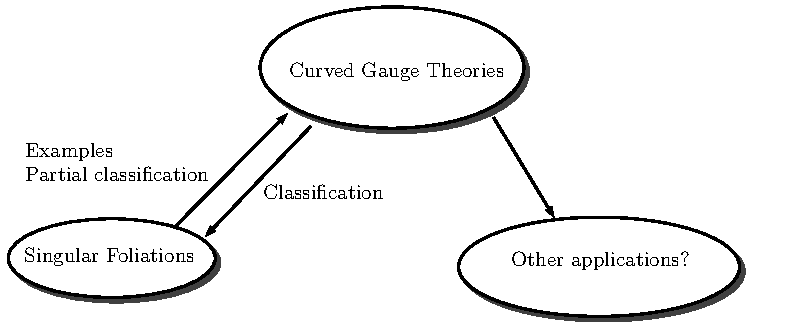
\includegraphics[width=1\textwidth]{Research circles I.pdf}
\end{figure}
\end{frame} 
}

\section[cYM]{Curved gauge theory}

\subsection{Motivation}
{
\setbeamertemplate{footline}
{
  \leavevmode%
  \hbox{%
  \begin{beamercolorbox}[wd=.09\paperwidth,ht=2.25ex,dp=1ex,center]{author in head/foot}%
    \usebeamerfont{author in head/foot}
		Sources
  \end{beamercolorbox}%
  \begin{beamercolorbox}[wd=.91\paperwidth,ht=2.25ex,dp=1ex,center]{title in head/foot}%
    \usebeamerfont{title in head/foot}
		Sombrero hat potential made by Mark J.D.\ Hamilton.
  \end{beamercolorbox}%
  %\begin{beamercolorbox}[wd=.175\paperwidth,ht=2.25ex,dp=1ex,right]{date in head/foot}%
    %\usebeamerfont{date in head/foot}\insertshortdate{}\hspace*{2em}
    %%\insertframenumber{} 
		%%/ \inserttotalframenumber\hspace*{2ex} 
  %\end{beamercolorbox}
	}%
  \vskip0pt%
}
\begin{frame}{\textbf{Infinitesimal} curved Yang-Mills-Higgs gauge theory}
\centering
\begin{tikzpicture}
\filldraw [fill=gray!10!white, draw=black] plot [smooth cycle] coordinates {(5,0.25) (6,0.35) (6.5, 0.2) (7,0.5) (7,1.65) (6.5,2.75) (5.8,2.75) (5.3,1.45) (4.8,0.85) } node at (6.2,1.7) {$(N, g)$} node at (6.2, 3.2) {Riemannian manifold};
\path[->] (2.6,1.7) edge [bend left] node[above] {Higgs field} node[below] {$\Psi$} (5.0,1.7);

\filldraw [fill=gray!10!white, draw=black] (-0.2,.5) to[bend left] (1.3,2.85) to[bend left] (2.7,2) to[bend right] (1.8,.5) to[bend right] cycle node at (1.2,1.7) {$(L, \eta)$} node at (1.2, 3.2) {Spacetime};
\path[->] (0.7,0.5) edge [bend right] node[left] {$A \in \Omega^1$} node[right] {Gauge bosons} (0.7, -1.5);
\filldraw [fill=gray, draw=black] (5.2, .7) circle (0.2);
\path[->] (2.5,-1.5) edge [bend right] node[right] {action $\gamma$} (5.2, .7);
\draw (-0.2,-1.7)-- (1.25, -1.7) node[below] {Lie algebra $\mathfrak{g}$} --(2.7,-1.7);

\tikzset{shift={(5,-3)}} %Change position of the next drawing
\begin{axis}[ scale = 0.6,
            hide axis,
            %axis lines=middle,
%            axis on top,
%            axis line style={blue,dashed,thick},
%            ymin=-2,ymax=2,
%            xmin=-2,xmax=2,
%            zmin=-2,zmax=2,
            samples=40,
            domain=0:360,
            y domain=0:1.25,clip=false
        ]
        \addplot3 [surf, shader=flat, draw=black, fill=gray!10!white, z buffer=sort]
           ({sin(x)*y}, {cos(x)*y}, {(y^2-1)^2});
        \draw[blue,thick,dashed] (axis cs:0,0,0) -- (axis cs:1,0,0)
                    node[below,font=\footnotesize]{};
        \draw[blue,thick,-stealth] (axis cs:1,0,0) -- (axis cs:1.3,0,0)
                    node[above,font=\footnotesize]{};
        \draw[blue,thick,dashed] (axis cs:0,0,0) -- (axis cs:0,-1,0)
                    node[left=2mm,font=\footnotesize]{}; %{Label} am Ende 
        \draw[blue,thick,-stealth] (axis cs:0,-1,0) -- (axis cs:0,-1.5,0)
                    node[right=1mm,font=\footnotesize]{};
        \draw[blue,thick,dashed] (axis cs:0,0,0) -- (axis cs:0,0,1)
                    %node[left=2mm,font=\footnotesize]{$\phi_{\text{RE}}$}
                    ;
        \draw[blue,thick,-stealth] (axis cs:0,0,1) -- (axis cs:0,0,1.3)
                    node[right,font=\footnotesize]{$\mathcal{V}$};
        \end{axis}
\end{tikzpicture}

\end{frame}

}

{
\setbeamertemplate{footline}{}

\begin{frame}{Motivation 1 by Thomas Strobl and Alexei Kotov}
\setbeamercovered{invisible}
\begin{table}[h!]
		\begin{tabularx}{\textwidth}{X X}
			\rowcolor{gray}
			Classical formalism & CYMH GT \\
			Lie algebra $\mathfrak{g}$ as $L \times \mathfrak{g}$ & Lie algebroid $E \to N$ \\
			\rowcolor{Gray}
			$\mathfrak{g}$-action $\gamma$ & Anchor $\rho$ of $E$ \\ 
			\rowcolor{Gray}
			& \& $E$-connections \\
			Canonical flat connection $\nabla^0$ on $L \times \mathfrak{g}$ & General connection $\nabla$ on $E$
		\end{tabularx}
\end{table}
\pause
\begin{remark}[Why a "curved theory"?]
Usually, the field strength $F$ is given by (abelian, for simplicity)
\bas
F
&\coloneqq
\mathrm{d}A
=
\mathrm{d}^{\nabla^0}A.
\eas
$\rightsquigarrow$ We will use a general connection $\nabla$ instead of $\nabla^0$, and $\nabla$ may not be flat.
\end{remark}
\end{frame}



}



%\subsection{Field Redefinition}
{
\setbeamertemplate{footline}{}

\begin{frame}{Motivation 2 by S.-R.\ F.}
Consider a semisimple Lie group $G$ and a principal $G$-bundle $P \to L$:
%$\mathbb{H}$ the horizontal distribution on $\mathcal{P} \tilde{\times} \mathcal{T}$:
\begin{center}
	\begin{tikzcd}[ampersand replacement=\&]
	(P \times \mathfrak{g})/G
	\arrow[hook]{r}
	\&
	\mathup{T}P/G
	\arrow[two heads]{r}
	\&
	\mathrm{T}L \arrow[bend right, swap]{l}{A}
	\end{tikzcd}
\end{center}
 
	%where $\mathup{Ad}(P)$ and $\mathup{At}(P)$ the adjoint and Atiyah bundle of a principal $G$-bundle $P$, respectively. 
	\pause
	\begin{gedankenexperiment}
	\begin{enumerate}
		\item Adjoint connection $\leftrightarrow$ Ehresmann connection on $P$. 
		\item Adjoint connection:
		\begin{equation*}
		\nabla_X \nu
		\coloneqq
		\mleft[ A(X), \nu \mright]_{\mathup{T}P/G}
		\end{equation*}
		for all $X \in \mathfrak{X}(L)$ and $\nu \in \Gamma((P \times \mathfrak{g})/G)$.
	\end{enumerate}
	\end{gedankenexperiment}
\end{frame}

\begin{frame}{Motivation 2 by S.-R.\ F.}
Consider a semisimple Lie group $G$ and a principal $G$-bundle $P \to L$:
%$\mathbb{H}$ the horizontal distribution on $\mathcal{P} \tilde{\times} \mathcal{T}$:
\begin{center}
	\begin{tikzcd}[ampersand replacement=\&]
	(P \times \mathfrak{g})/G
	\arrow[hook]{r}
	\&
	\mathup{T}P/G
	\arrow[two heads]{r}
	\&
	\mathrm{T}L \arrow[bend right, swap]{l}{A}
	\end{tikzcd}
\end{center}
 
	%where $\mathup{Ad}(P)$ and $\mathup{At}(P)$ the adjoint and Atiyah bundle of a principal $G$-bundle $P$, respectively. 
	
	\begin{gedankenexperiment}
	\begin{enumerate}
		\item Adjoint connection $\leftrightarrow$ Ehresmann connection on $P$. 
		\item As parallel transport:
		\begin{equation*}
		\mathup{PT}_\gamma^{\mathup{Ad}(P)}([p, v])
		=
		\mleft[ \mathup{PT}_\gamma^P(p), v \mright]
		\end{equation*}
		for all $[p, v] \in (P \times \mathfrak{g})/G$.
	\end{enumerate}
	\end{gedankenexperiment}
\end{frame}

\begin{frame}{Motivation 2 by S.-R.\ F.}
Consider a semisimple Lie group $G$ and a principal $G$-bundle $P \to L$:
%$\mathbb{H}$ the horizontal distribution on $\mathcal{P} \tilde{\times} \mathcal{T}$:
\begin{center}
	\begin{tikzcd}[ampersand replacement=\&]
	\mleft(P \times_L \underline{\mathfrak{g}}\mright)/G
	\arrow[hook]{r}
	\&
	\mathup{T}P/G
	\arrow[two heads]{r}
	\&
	\mathrm{T}L \arrow[bend right, swap]{l}{A}
	\end{tikzcd}
\end{center}
 
	%where $\mathup{Ad}(P)$ and $\mathup{At}(P)$ the adjoint and Atiyah bundle of a principal $G$-bundle $P$, respectively. 
	
	\begin{gedankenexperiment}
	\begin{enumerate}
		\item Adjoint connection $\leftrightarrow$ Ehresmann connection on $P$. 
		\item As parallel transport:
		\begin{equation*}
		\mathup{PT}_\gamma^{\mathup{Ad}(P)}([p, v])
		=
		\mleft[ \mathup{PT}_\gamma^P(p), \mathup{PT}_\gamma^0(v) \mright],
		\end{equation*}
		Lie algebra $\mathfrak{g}$ as trivial bundle w/ canonical flat connection
	\end{enumerate}
	\end{gedankenexperiment}
\end{frame}

\begin{frame}{Motivation 2 by S.-R.\ F.}
Consider a semisimple Lie group $G$ and a principal $G$-bundle $P \to L$:
%$\mathbb{H}$ the horizontal distribution on $\mathcal{P} \tilde{\times} \mathcal{T}$:
\begin{center}
	\begin{tikzcd}[ampersand replacement=\&]
	\mleft(P \times_L \underline{\mathfrak{g}}\mright)/G
	\arrow[hook]{r}
	\&
	\mathup{T}P/G
	\arrow[two heads]{r}
	\&
	\mathrm{T}L \arrow[bend right, swap]{l}{A}
	\end{tikzcd}
\end{center}
 
	%where $\mathup{Ad}(P)$ and $\mathup{At}(P)$ the adjoint and Atiyah bundle of a principal $G$-bundle $P$, respectively. 
	
	\begin{gedankenexperiment}
	\begin{enumerate}
		\item Adjoint connection $\leftrightarrow$ Ehresmann connection on $P$. 
		\item As parallel transport:
		\begin{equation*}
		\mathup{PT}_\gamma^{\mathup{Ad}(P)}([p, v])
		=
		\mleft[ \mathup{PT}_\gamma^P(p){\color[rgb]{0.24,0.7,0.44} \cdot \kappa_\gamma}, {\color[rgb]{0.24,0.7,0.44} \kappa_\gamma^{-1} \cdot} \mathup{PT}_\gamma^0(v) \mright],
		\end{equation*}
		Lie algebra $\mathfrak{g}$ as trivial bundle w/ canonical flat connection, $\kappa_\gamma$ values in $G$ \& "suitable"
	\end{enumerate}
	\end{gedankenexperiment}
\end{frame}


\begin{frame}
\begin{theorem}[Field Redefinitions {S.-R.\ F.}]
%\begin{itemize}[<+->]
This leads to an equivalence relation of gauge theories, preserving dynamics and kinematics.

But: In the {\color[rgb]{0.24,0.7,0.44} curved} sense! Curvature terms appear.
\end{theorem}
\pause
\begin{motivation}[{S.-R.\ F.}]
\begin{enumerate}
	\item How to formulate gauge theory such that it is invariant under field redefinitions?
	\item Are there curved theories which are \textbf{not} equivalent to classical ones?
\end{enumerate}
\end{motivation}


\end{frame}

}

\subsection{Principal bundle}

{
\setbeamertemplate{footline}{}
\begin{frame}
\textbf{We will only focus on Yang-Mills theories:}

\begin{table}[h!]
		\begin{tabularx}{\textwidth}{X| c c} 
			\rowcolor{gray}
			& Classical & Curved \\ \hline
			Infinitesimal & Lie algebra $\mathfrak{g}$ & LAB\footnote{LAB = Lie algebra bundle} $\mathcal{g}$ \\
			\rowcolor{Gray}
			Integrated & Lie group $G$ & \textcolor[rgb]{1,0.41,0.13}{LGB\footnote{LGB = Lie group bundle} $\mathcal{G}$} \\
		\end{tabularx}
\end{table}

\begin{center}
	\begin{tikzcd}[ampersand replacement=\&]
	G \arrow{r} \& \mathcal{G} \arrow{d} \\
	\& M
	\end{tikzcd}
\end{center}

\end{frame}
}

\renewcommand\insertreferences{{\tiny  K. Mackenzie. General Theory of Lie Groupoids and Algebroids. \newline \textit{London Mathematical Society Lecture Note Series}, 213, 2005.}}

\begin{frame}
\begin{definition}[LGB actions, simplified]
\begin{center}
	\begin{tikzcd}[ampersand replacement=\&, column sep = small, row sep = small]
	\& \arrow[bend right]{ld} \mathcal{G} \arrow{d} \\
	\mathcal{P} \arrow{r}{\pi} \& L
	\end{tikzcd}
\end{center}
$\mathcal{P} \stackrel{\pi}{\to} L$ a fibre bundle. A \textbf{right-action of $\mathcal{G}$ on $\mathcal{P}$} is a smooth map 
%\bas
$\mathcal{P} * \mathcal{G} \coloneqq \pi^*\mathcal{G} = \mathcal{P} \times_L \mathcal{G} \to \mathcal{P}$,
$(p, g) \mapsto p \cdot g$,
%\eas
satisfying the following properties:
\ba\label{InvarianceOffUnderGAction}
\pi(p \cdot g) &= \pi(p),\\
(p \cdot g) \cdot h &= p \cdot (gh),\\
p \cdot e_{\pi(p)} &= p
\ea
for all $p \in \mathcal{P}$ and $g, h \in \mathcal{G}_{\pi(p)}$, where $e_{\pi(p)}$ is the neutral element of $\mathcal{G}_{\pi(p)}$.
\end{definition}
\end{frame}


\renewcommand\insertreferences{{\tiny Ieke Moerdijk, Janez Mrcun. Introduction to Foliations and Lie Groupoids. \newline \textit{Cambridge Studies in Advanced Mathematics 91, Cambridge University Press, Cambridge}, 2003}}

\begin{frame}
\begin{definition}[Principal bundle]
Still a fibre bundle
\begin{center}
	\begin{tikzcd}[ampersand replacement=\&]
	G \arrow{r} \& \mathcal{P} \arrow{d}{\pi} \\
	\& L
	\end{tikzcd}
\end{center}
but with $\mathcal{G}$-action
\bas
\begin{matrix}
	\textcolor[rgb]{1,0,0}{\xcancel{\mathcal{P} \times G}} &\to \mathcal{P} \\
	\mathcal{P} * \mathcal{G} &
\end{matrix}
\eas
simply transitive on fibres of $\mathcal{P}$, and "suitable" atlas.
\end{definition}
\end{frame}

\subsection{Connections as parallel transport}
{
\setbeamertemplate{footline}{}
\begin{frame}{Connection on $\mathcal{P}$: Idea}
\begin{figure}
%\caption{Pushforwards via right-multiplication of tangent vectors}  
%\label{figure:fibre bundle}
\centering
\begin{tikzpicture}[scale=0.55]
\draw (0,-3.5) to[out=10,in=170] (4.25,-3.5) to[out=350,in=190] (8.5,-3.5);
\draw (1.25,2.5) to[out=280,in=90](1.5,0) to[out=270,in=80] (1.25,-2.5);
\filldraw [fill=gray!20!white, draw=white] (3.5,2.5) to[out=280,in=90](3.75,0) to[out=270,in=80] (3.5,-2.5) -- (5,-2.5)  to[out=80,in=270](5.25,0) to[out=90,in=280] (5,2.5) -- cycle;
\draw (4.25,2.5) to[out=280,in=95](4.41,1) to[out=275,in=85] (4.41,-1) to[out=265,in=80] (4.25,-2.5); %draw with middle section for precise point placement

\draw (4,-1) node {\textcolor[rgb]{1,0,0}{$p$}};
\draw [<-, draw=blue] (5,1) to[out=275,in=85] (5,-1);
\draw (5.5,0) node {\textcolor[rgb]{0,0,1}{$\cdot g$}};
\filldraw [fill=red, draw=red] (4.41,1) circle (1pt);
\filldraw [fill=red, draw=red] (4.41,-1) circle (1pt);
\draw (5.75,2.5) to[out=280,in=90](6,0) to[out=270,in=80] (5.75,-2.5);
\draw (7.25,2.5) to[out=280,in=90](7.5,0) to[out=270,in=80] (7.25,-2.5);
\draw (2.75,2.475) to[out=280,in=90](3,0) to[out=270,in=80] (2.75,-2.475);

%\draw (4.75,2) node {$\mathcal{P}_x$};
%\draw (4.95,1.5) node {$\cong G$};
\draw (9.5,-3.5) node {$L$};
\draw (5,2) node {$\mathcal{P}_U$};
\draw (3.5,-3.4) node {$($};
\filldraw [fill=red, draw=red] (4.25,-3.5) circle (1pt);
\draw (4.25,-3.9) node {\textcolor[rgb]{1,0,0}{$x$}};
\draw (5,-3.6) node {$)$};
\draw (4.25, -3) node {$U$};
\draw (0,0) node {$\mathcal{P}$};
\draw [->] (0,-0.4) -- (0,-3.1);
\draw (0.4,-1.75) node {$\pi$};
\draw (3.5,1) node {\textcolor[rgb]{1,0,0}{$p \cdot g$}};
%%%%%%%%%%%%%%%%%%%%%%%%%%%%%%%%%%%%%%%%%%%%%%%%%%%%%%%%%%%%%%%%%%%%%%%%%%%%%%%%%%%%
\draw (10.5,-3.5) to[out=10,in=170] (14.75,-3.5) to[out=350,in=190] (19,-3.5); %hori M
\filldraw [fill=gray!20!white, draw=white] (14,2.5) to[out=280,in=90](14.25,0) to[out=270,in=80] (14,-2.5) -- (15.5,-2.5)  to[out=80,in=270](15.75,0) to[out=90,in=280] (15.5,2.5) -- cycle; %gray area
\draw (11.75,2.5) to[out=280,in=90](12,0) to[out=270,in=80] (11.75,-2.5); %vert line 1
\draw (14.75,2.5) to[out=280,in=90](15,0) to[out=270,in=80] (14.75,-2.5); %3
\draw (16.25,2.5) to[out=280,in=90](16.5,0) to[out=270,in=80] (16.25,-2.5); %4
\draw (17.75,2.5) to[out=280,in=90](18,0) to[out=270,in=80] (17.75,-2.5); %5

\draw (13.25,2.475) to[out=280,in=90](13.5,0) to[out=270,in=80] (13.25,-2.475); %2
\filldraw [fill=blue, draw=blue] (15,0) circle (1pt);
\draw (15.5,0) node {\textcolor[rgb]{0,0,1}{$g$}};

\draw (19,0) node {$\mathcal{G}$}; %These three lines are for LGB projection
\draw [->] (19,-0.4) -- (19,-3.1);
%\draw (18.5,-1.75) node {$\pi_{\mathcal{G}}$};

\draw (15.5,2) node {$\mathcal{G}_U$};
\draw (14,-3.4) node {$($};
\filldraw [fill=red, draw=red] (14.75,-3.5) circle (1pt);
\draw (14.75,-3.9) node {\textcolor[rgb]{1,0,0}{$x$}};
\draw (15.5,-3.6) node {$)$};
\draw (14.75, -3) node {$U$};

\path[<-] (8.5,0) edge [bend left] (11,0);
\end{tikzpicture}
\end{figure}
\pause
But:
\bas
&&&r_g: \mathcal{P}_x \to \mathcal{P}_x\\
&\Rightarrow&&\mathrm{D}_pr_g \text{ only defined on vertical structure}
\eas
\end{frame}

\begin{frame}{Connection on $\mathcal{P}$: Idea}
\begin{figure}
%\caption{Pushforwards via right-multiplication of tangent vectors}  
%\label{figure:fibre bundle part two}
\centering
\begin{tikzpicture}[scale=0.55]
\draw (0,-3.5) to[out=10,in=170] (4.25,-3.5) to[out=350,in=190] (8.5,-3.5);
\draw (1.25,2.5) to[out=280,in=90](1.5,0) to[out=270,in=80] (1.25,-2.5);
\filldraw [fill=gray!20!white, draw=white] (3.5,2.5) to[out=280,in=90](3.75,0) to[out=270,in=80] (3.5,-2.5) -- (5,-2.5)  to[out=80,in=270](5.25,0) to[out=90,in=280] (5,2.5) -- cycle;
\draw (4.25,2.5) to[out=280,in=95](4.41,1) to[out=275,in=85] (4.41,-1) to[out=265,in=80] (4.25,-2.5); %draw with middle section for precise point placement

\draw (4,-1) node {\textcolor[rgb]{1,0,0}{$p$}};
\draw [<-, draw=blue] (5,1) to[out=275,in=85] (5,-1);
\draw [<-, draw=blue] (4.8,1) to[out=275,in=85] (4.8,-1);
\draw [<-, draw=blue] (4.6,1) to[out=275,in=85] (4.6,-1);
\draw (5.5,0) node {\textcolor[rgb]{0,0,1}{$\cdot \sigma$}};
\filldraw [fill=red, draw=red] (4.41,1) circle (1pt);
\filldraw [fill=red, draw=red] (4.41,-1) circle (1pt);
\draw (5.75,2.5) to[out=280,in=90](6,0) to[out=270,in=80] (5.75,-2.5);
\draw (7.25,2.5) to[out=280,in=90](7.5,0) to[out=270,in=80] (7.25,-2.5);
\draw (2.75,2.475) to[out=280,in=90](3,0) to[out=270,in=80] (2.75,-2.475);

%\draw (4.75,2) node {$\mathcal{P}_x$};
%\draw (4.95,1.5) node {$\cong G$};
\draw (9.5,-3.5) node {$L$};
\draw (5,2) node {$\mathcal{P}_U$};
\draw (3.5,-3.4) node {$($};
\filldraw [fill=red, draw=red] (4.25,-3.5) circle (1pt);
\draw (4.25,-3.9) node {\textcolor[rgb]{1,0,0}{$x$}};
\draw (5,-3.6) node {$)$};
\draw (4.25, -3) node {$U$};
\draw (0,0) node {$\mathcal{P}$};
\draw [->] (0,-0.4) -- (0,-3.1);
\draw (0.4,-1.75) node {$\pi$};
\draw (3.5,1) node {\textcolor[rgb]{1,0,0}{$p \cdot \sigma_x$}};
%%%%%%%%%%%%%%%%%%%%%%%%%%%%%%%%%%%%%%%%%%%%%%%%%%%%%%%%%%%%%%%%%%%%%%%%%%%%%%%%
\draw (10.5,-3.5) to[out=10,in=170] (14.75,-3.5) to[out=350,in=190] (19,-3.5); %hori M
\filldraw [fill=gray!20!white, draw=white] (14,2.5) to[out=280,in=90](14.25,0) to[out=270,in=80] (14,-2.5) -- (15.5,-2.5)  to[out=80,in=270](15.75,0) to[out=90,in=280] (15.5,2.5) -- cycle; %gray area
\draw (11.75,2.5) to[out=280,in=90](12,0) to[out=270,in=80] (11.75,-2.5); %vert line 1
\draw (14.75,2.5) to[out=280,in=90](15,0) to[out=270,in=80] (14.75,-2.5); %3
\draw (16.25,2.5) to[out=280,in=90](16.5,0) to[out=270,in=80] (16.25,-2.5); %4
\draw (17.75,2.5) to[out=280,in=90](18,0) to[out=270,in=80] (17.75,-2.5); %5

\draw (13.25,2.475) to[out=280,in=90](13.5,0) to[out=270,in=80] (13.25,-2.475); %2
\draw [draw=blue] (14.25,0) to[out=10,in=170] (15,0) to[out=350,in=190] (15.75,0);
%\filldraw [fill=blue, draw=blue] (15,0) circle (1pt);
\draw (13.9,0) node {\textcolor[rgb]{0,0,1}{$\sigma$}};

\draw (19,0) node {$\mathcal{G}$}; %These three lines are for LGB projection
\draw [->] (19,-0.4) -- (19,-3.1);
%\draw (18.5,-1.75) node {$\pi_{\mathcal{G}}$};

\draw (15.5,2) node {$\mathcal{G}_U$};
\draw (14,-3.4) node {$($};
\filldraw [fill=red, draw=red] (14.75,-3.5) circle (1pt);
\draw (14.75,-3.9) node {\textcolor[rgb]{1,0,0}{$x$}};
\draw (15.5,-3.6) node {$)$};
\draw (14.75, -3) node {$U$};

\path[<-] (8.5,0) edge [bend left] (11,0);
\end{tikzpicture}
\end{figure}

\bas
\text{Use } \sigma \in \Gamma(\mathcal{G}): r_\sigma(p) \coloneqq p \cdot \sigma_{x}
\eas
\end{frame}

\begin{frame}{Connection on $\mathcal{P}$: Revisiting the classical setup}
\setbeamercovered{invisible}
	\begin{minipage}[]{0.45\textwidth} 
	If $\mathcal{P}$ a typical principal bundle ($\mathcal{G}$ trivial, $\sigma \equiv g$ constant), and \textcolor[rgb]{0,0.58,0}{$H$} a connection:
	\begin{figure}
	\begin{tikzpicture}[scale=1.2]
		%Gray area
		\filldraw [fill=gray!20!white, draw=white] (3.5,2.5) to[out=280,in=95](3.66,1) to[out=275,in=85] (3.66,-1) to[out=265,in=80] (3.5,-2.5) -- (5,-2.5) to[out=80, in=265] (5.16, -1) to[out=85, in=275] (5.16, 1) to[out=95,in=280] (5,2.5) -- cycle;
		%lines
		\draw (4.25,2.5) to[out=280,in=95](4.41,1) to[out=275,in=85] (4.41,-1) to[out=265,in=80] (4.25,-2.5);
		\definecolor{darkgreen}{rgb}{0,0.58,0}
		\draw [draw=darkgreen] (3.66,-1) to[out=280,in=200] (4.41,-1) to[out=20,in=100] (5.16, -1);
		\draw [draw=darkgreen] (3.66,1) to[out=280,in=200] (4.41,1) to[out=20,in=100] (5.16,1);
		%Auxiliary stuff like arrows and dots
		\filldraw [fill=red, draw=red] (4.41,1) circle (1pt);
		\filldraw [fill=red, draw=red] (4.41,-1) circle (1pt);
		\draw [<-, draw=blue] (5.16,1) to[out=275,in=85] (5.16,-1);
		\draw [->, thick] (4.41,-1) -- (4.71,-0.88);
		%\draw [->] (4.41,1) -- (4.63,2);
		\draw [->, thick] (4.41,1) -- (4.71,1.12);
		%\draw [<-,dotted,thick] (4.63,2) -- (4.71,1.12);
		%Labels
		\draw (3.2,1) node {\textcolor[rgb]{0,0.58,0}{$H_{p \cdot g}$}};
		\draw (3.2,-1) node {\textcolor[rgb]{0,0.58,0}{$H_p$}};
		\draw (5.5,0) node {\textcolor[rgb]{0,0,1}{$\cdot g$}};
		\draw (3,2.2) node {$\mathcal{P}_U$};
		\draw (4.71,-0.6) node {$X$};
		\draw (5,1.4) node {$\mathrm{D}_pr_g(X)$};
		%\draw (5.5,1.56) node {$\thicksim \mathrm{D}_x\sigma(X)$};
		%Text
	\end{tikzpicture}
	\end{figure}
	\end{minipage}\hfill
	\pause
	\begin{minipage}[]{0.45\textwidth} 
	\begin{remark}[Integrated case]
	Parallel transport $\mathup{PT}^{\mathcal{P}}_\gamma$ in $\mathcal{P}$:
		\bas
		%\mathrm{D}_p r_g (X)
		%&=
		%\mleft.\frac{\mathrm{d}}{\mathrm{d}t}\mright|_{t=0}\mleft( \alpha \cdot g \mright),
		\mathup{PT}^{\mathcal{P}}_\gamma(p \cdot g)
		&=
		\mathup{PT}^{\mathcal{P}}_\gamma(p) \cdot g
		%\\
		%&=
		%\mathup{PT}^{\mathcal{P}}_\alpha(p) \cdot \mathup{PT}^{\mathcal{G}}_\alpha (g)
		\eas
		where $\gamma:I \to L$ is a base path 
	\end{remark}
	\end{minipage}
\end{frame}
%
%{
%\setbeamertemplate{footline}{}

\begin{frame}{Connection on $\mathcal{P}$: General case}
	\begin{remark}[Integrated case]
	Ansatz: Introduce connection on $\mathcal{G}$,
		\bas
		\mathup{PT}^{\mathcal{P}}_\gamma(p \cdot g)
		&=
		\mathup{PT}^{\mathcal{P}}_\gamma(p) \cdot \mathup{PT}^{\mathcal{G}}_{\gamma} (g).
		\eas
	\end{remark}
	\pause
\begin{BackToTheRoots}
\begin{enumerate}
	\item $\mathcal{G} \cong L \times G$
	\item Equip $\mathcal{G}$ with canonical flat connection
\end{enumerate}
\end{BackToTheRoots}
\end{frame}
%\subsection{General notion of Ehresmann and Yang-Mills connections}
\begin{frame}
\begin{definition}[Ehresmann/Yang-Mills connection, {[C.\ L.-G., S.-R.\ F.]}]
A surjective submersion $\pi_{\mathcal{T}} \colon \mathcal{T} \to L$ so that one has a commuting diagram
\begin{center}
	\begin{tikzcd}[ampersand replacement=\&]
	\& \arrow[bend right]{ld} \mathcal{G} \arrow{d}{\pi_{\mathcal{G}}}
    %\arrow{l} G 
    \\
	\mathcal{T} \arrow{r}{\pi_{\mathcal{T}}} \& L
	\end{tikzcd}
\end{center}
\begin{enumerate}
	\item \textbf{Ehresmann connection:} 
	\bas
	\mathup{PT}_\gamma^{\mathcal{T}}(t \cdot g)
	&=
	\mathup{PT}_\gamma^{\mathcal{T}}(t)
	\cdot
	\mathup{PT}_{\gamma}^{\mathcal{G}}(g)
	\eas
	\item \textbf{Yang-Mills connection:} Additionally
	\bas
	\mathup{PT}_{\gamma_0}^{\mathcal{T}}(t)
	&=
	t \cdot g_{\gamma_0}
	\eas
	for some $g_{\gamma_0} \in \mathcal{G}_{\pi_{\mathcal{T}}(t)}$, where $\gamma_0$ is a contractible loop.
\end{enumerate}
\end{definition}
\end{frame}

\begin{frame}
\begin{definition}[Multiplicative YM connection, {[S.-R.\ F.]}]
On $\mathcal{G}$ there is also the notion of \textbf{multiplicative Yang-Mills connections}, that is,
\bas
\mathup{PT}_\gamma^{\mathcal{G}}(q \cdot g)
&=
\mathup{PT}_\gamma^{\mathcal{G}}(q)
\cdot
\mathup{PT}_{\gamma}^{\mathcal{G}}(g),
\\
\mathup{PT}_{\gamma_0}^{\mathcal{G}}(q)
&=
g_{\gamma_0} \cdot q \cdot g_{\gamma_0}^{-1}
\eas
\end{definition}
\end{frame}
}
%
%\subsection{Connection and curvature}
%
%{
%\setbeamertemplate{footline}{}

\renewcommand\insertreferences{{\tiny For differential: Marius Crainic, Maria Amelia Salazar, and Ivan Struchiner. Multiplicative forms and Spencer operators. \newline \textit{Mathematische Zeitschrift}, 279(3):939–979, 2015.}}

\begin{frame}
\begin{remark}
There is a simplicial differential $\delta$ on $\mathcal{G} \stackrel{\pi_{\mathcal{G}}}{\to} L$ with Lie algebra bundle $\mathcal{g}$
\bas
\delta: \Omega^\bullet( \underbrace{\mathcal{G} * \dotsc * \mathcal{G}}_{k \text{ times}}; \pi_{\mathcal{G}}^*\mathcal{g} )
&\to
\Omega^\bullet( \underbrace{\mathcal{G} * \dotsc * \mathcal{G}}_{k + 1 \text{ times}}; \pi_{\mathcal{G}}^*\mathcal{g} )
\eas
such that the definition of the multiplicative Yang-Mills connection is equivalent to the \textbf{compatibility conditions}
\begin{itemize}
	\item Connection closed
	\item Curvature exact ([S.-R.\ F.])
\end{itemize}
\end{remark}
\end{frame}

\renewcommand\insertreferences{{\tiny For the first equation: Camille Laurent-Gengoux, Mathieu Stiénon, and Ping Xu. Non-abelian differentiable gerbes. \newline \textit{Advances in Mathematics}, 220(5):1357–1427, 2009.}}

\begin{frame}
\begin{remark}
On the Lie algebra bundle $\mathcal{g}$ we have a connection $\nabla$ with 
\bas
\nabla\mleft( \mleft[ \mu, \nu \mright]_{\mathcal{g}} \mright)
&=
\mleft[ \nabla \mu, \nu \mright]_{\mathcal{g}}
	+ \mleft[ \mu, \nabla \nu \mright]_{\mathcal{g}},
\\
R_{\nabla}
&=
\mathrm{ad} \circ \zeta.
\eas
\end{remark}
\pause
\begin{example}
Given a short exact sequence of algebroids 
\begin{center}
	\begin{tikzcd}[ampersand replacement=\&]
	\mathcal{g} \arrow[hook]{r}
	\& E \arrow[two heads]{r}
	\& \mathrm{T}L \arrow[bend right, swap]{l}{A}
	\end{tikzcd}
\end{center}
with splitting $A \colon \mathrm{T}L \to E$, then
\bas
\nabla_X \nu
&=
\mleft[ A(X), \nu \mright]_E,
\\
\zeta\mleft( X, X' \mright)
&=
\mleft[ A(X), A(X') \mright]_E
	- A\mleft( [X, X'] \mright).
\eas
\end{example}
\end{frame}

\subsection{Field strength}

{
\setbeamertemplate{footline}{}
\begin{frame}{Integrating Alexei Kotov's and Thomas Strobl's idea}
%Given a multiplicative Yang-Mills connection on $\mathcal{G}$:

\begin{definition}[Principal bundle connection, {[S.-R.\ F.]}]
\begin{itemize}
	\item On $\mathcal{G}$: Multiplicative Yang-Mills connection
	\item On $\mathcal{P}$: Ehresmann connection
\end{itemize}
\end{definition}

\pause

\begin{definition}[Generalized curvature/field strength $F$ of $A$, {[S.-R.\ F.]}]
We define
\bas
F
&\coloneqq
\mathrm{d}^{\pi^*\nabla} A
	+ \frac{1}{2} \mleft[ A \stackrel{\wedge}{,} A \mright]_{\pi^*\mathcal{g}}
	+ \pi^!\zeta.
\eas
\end{definition}
\end{frame}
}

\subsection{Curved Yang-Mills gauge theory}

{
\setbeamertemplate{footline}{}

\begin{frame}
\begin{theorem}[Lagrangian, {[S.-R.\ F.]}]
\begin{itemize}
	\item $\kappa$ be an $\mathrm{Ad}$-invariant fibre metric on $\mathcal{g}$, 
	\item $L$ a spacetime, and $*$ its Hodge star operator, 
	\item $\mleft( U_i \mright)_i$ open covering of $L$ with subordinate gauges $s_i \in \Gamma\mleft(\mathcal{P}|_{U_i}\mright)$.
\end{itemize}
Then the Lagrangian $\mathfrak{L}_{\mathrm{CYM}}[A]$, defined locally by
\bas
\mleft.\bigl(\mathfrak{L}_{\mathrm{CYM}}[A]\bigr)\mright|_{U_i}
&\coloneqq 
- \frac{1}{2} \kappa \mleft( F_{s_i} \stackrel{\wedge}{,} *F_{s_i} \mright),
\eas
is well-defined, and
\bas
\mathfrak{L}_{\mathrm{CYM}}\mleft[ K^!A \mright]
&=
\mathfrak{L}_{\mathrm{CYM}}[A]
\eas
for all principal bundle automorphisms $K$.
\end{theorem}
\end{frame}

\subsection{Classical theory}

\begin{frame}
\begin{BackToTheRoots}
\begin{enumerate}
	\item $\mathcal{G} \cong L \times G$
	\item Equip $\mathcal{G}$ with canonical flat connection
	%\pause
	\item $\zeta \equiv 0$
\end{enumerate}
\end{BackToTheRoots}
\end{frame}

\subsection{Example}

\begin{frame}
\begin{example}[Hopf fibration $\mathds{S}^7 \to \mathds{S}^4$, {[S.-R.\ F.]}]
Let $P$ be the Hopf bundle
\begin{center}
	\begin{tikzcd}[ampersand replacement=\&, column sep=small]
		\mathrm{SU}(2) \cong \mathds{S}^3 \arrow{r}	\& \mathds{S}^7 \arrow{d} \\
			\& \mathds{S}^4
	\end{tikzcd}
\end{center}
Define $\mathcal{P} \coloneqq \mathcal{G}$ as the inner group bundle of $P$,
\bas
\mathcal{G}
&\coloneqq
c_{\mathrm{SU}(2)}(P)
\coloneqq 
\bigl(P\times \mathrm{SU}(2)\bigr) \Big/ \mathrm{SU}(2).
\eas
This principal $c_{\mathrm{SU}(2)}(P)$-bundle admits the structure as curved Yang-Mills gauge theory; there is no description as classical gauge theory.
\end{example}
\end{frame}

}


%\section[Classification]{An attempt of classification}
%
%
%{
%\setbeamertemplate{footline}{}
%\begin{frame}
%\begin{definition}[Field redefinition, {[S.-R. F.]}]
%Let $\lambda \in \Omega^1(L; \mathcal{g})$, then we define the \textbf{field redefinitions} by 
%\bas\label{EqFieldRedefFuerA}
%\widetilde{A}^\lambda
%&\coloneqq 
%A - \pi_{\mathcal{P}}^! \lambda,
%\\
%\widetilde{\nabla}^\lambda
%&\coloneqq
%\nabla
	%+ \mathrm{ad} \circ \lambda,
%\\
%\widetilde{\zeta}^\lambda
%&\coloneqq
%\zeta
	%+ \mathrm{d}^{\widetilde{\nabla}^\lambda} \lambda
	%+ \frac12 \mleft[ \lambda \stackrel{\wedge}{,} \lambda \mright]_{\mathcal{g}},
%\eas
%where $A \in \Omega^1(\mathcal{P}; \pi_{\mathcal{P}}^*\mathcal{g})$ is the connection 1-form on $\mathcal{P}$.
%%for all $X, Y \in \mathfrak{X}(L)$.
%\end{definition}
%\end{frame}
%
%\begin{frame}
%\begin{proposition}[{[S.-R. F.]}]
%\begin{itemize}
	%\item Field redefinitions define an equivalence relation of CYMH gauge theories
	%\item $\widetilde{\mathfrak{L}}^\lambda_{\mathrm{CYMH}} = \mathfrak{L}_{\mathrm{CYMH}}$
%\end{itemize}
%\end{proposition}
%%\vfill
%\pause
%Let us now apply a field redefinition in order to study whether $\nabla$ and $\zeta$ can become flat and zero, respectively.
%\end{frame}
%}
%
%%\subsection{Classification}
%
%{
%\setbeamertemplate{footline}{}
%\begin{frame}
%\begin{theorem}[Invariant for LABs, {[S.-R. F.]}]
%We have
%\bas
%\mathrm{d}^{\widetilde{\nabla}^\lambda} \widetilde{\zeta}^\lambda = \mathrm{d}^\nabla \zeta,
%\eas
%and $\mathrm{d}^\nabla \zeta$ has values in the centre of ${\mathcal{g}}$.
%\end{theorem}
%
%\begin{proof}
%Bianchi identity given by $\mathrm{d}^\nabla \zeta$.
%
%Compatibilities: 
%\bas
%\nabla_Y\mleft( \mleft[ \mu, \nu \mright]_{\mathcal{g}} \mright)
%&=
%\mleft[ \nabla_Y \mu, \nu \mright]_{\mathcal{g}}
	%+ \mleft[ \mu, \nabla_Y \nu \mright]_{\mathcal{g}}, \\
%R_\nabla(Y, Z) \mu
%&=
%\mleft[ \zeta(Y, Z), \mu \mright]_{\mathcal{g}}
%\eas
%for all $Y, Z \in \mathfrak{X}(N)$ and $\mu, \nu \in \Gamma({\mathcal{g}})$.
%\end{proof}
%\end{frame}
%
%\begin{frame}{Behaviour of the field redefinition of $\zeta$}
%\begin{theorem}[Existence of non-classical theories, {[S.-R. F.]}]
%If $\mathrm{d}^\nabla \zeta \neq 0$, then there is no field redefinition such that $\widetilde{\zeta}^\lambda = 0$.
%\end{theorem}
%\pause
%\begin{remark}[{[S.-R. F.]}]
%Starting with a classical theory:
%
%If $\mathrm{dim}(N) \geq 3$ and if Lie algebra $\mathfrak{g}$ has a non-zero centre, then we can always construct a pre-classical CYMH GT which is not a classical one by adding a $\zeta$ with $\mathrm{d}^\nabla \zeta \neq 0$.
%\end{remark}
%\pause
%However, by $R_\nabla = \mathrm{ad}_{\mathcal{g}} \circ \zeta$ it may still be that $\nabla$ becomes flat.
%\end{frame}
%
%\begin{frame}{Turning to the field redefinition of $\nabla$:}
%\begin{theorem}[Differential on centre-valued forms, {[S.-R. F.]}]
%$\nabla$ restricts to the centre of ${\mathcal{g}}$ and induces a differential $\mathrm{d}^\Xi$ on centre-valued forms. Moreover, $\mathrm{d}^\Xi$ is independent of the field redefinitions.
%\end{theorem}
%\pause
%\begin{proof}[Sketch of proof]
%Recall
%\bas
%\nabla_Y\mleft( \mleft[ \mu, \nu \mright]_{\mathcal{g}} \mright)
%&=
%\mleft[ \nabla_Y \mu, \nu \mright]_{\mathcal{g}}
	%+ \mleft[ \mu, \nabla_Y \nu \mright]_{\mathcal{g}}, \\
%R_\nabla(Y, Z) \mu
%&=
%\mleft[ \zeta(Y, Z), \mu \mright]_{\mathcal{g}}, \\
%\widetilde{\nabla}^\lambda_Y \mu
%&=
%\nabla_Y \mu
%- \mleft[\lambda(Y), \mu\mright]_{\mathcal{g}},
%\eas
%for all $Y, Z \in \mathfrak{X}(N)$ and $\mu, \nu \in \Gamma({\mathcal{g}})$. Then insert $\mu$ with values in the centre.
%\end{proof}
%\end{frame}
%
%\begin{frame}
%\begin{theorem}[Closedness of $\mathrm{d}^\nabla \zeta$, {[S.-R. F.]}]
%We have
%\bas
%\mathrm{d}^\Xi \mathrm{d}^\nabla \zeta
%&=
%0.
%\eas
%\end{theorem}
%\pause
%\begin{definition}[Obstruction class, {[S.-R. F.]}]
%We define the \textbf{obstruction class} by
%\bas
%\mathrm{Obs}(\Xi)
%&\coloneqq
%\mleft[ \mathrm{d}^\nabla \zeta \mright]_{\mathrm{d}^\Xi}.
%\eas
%\end{definition}
%\pause
%\begin{proposition}[{[S.-R. F.]}]
%\begin{itemize}[<+->]
	%\item An invariant of the field redefinitions.
	%\item If $\nabla$ flat, then $\mathrm{Obs}(\Xi) = 0$.
%\end{itemize}
%\end{proposition}
%\end{frame}
%
%\begin{frame}
%\begin{theorem}[Obstruction for non-pre-classical theories, {[S.-R. F.]}]
%If $\mathrm{Obs}(\Xi) \neq 0$, then there is no field redefinition such that $\widetilde{\nabla}^\lambda$ is flat.
%\end{theorem}
%\pause
%\begin{theorem}[Locally always pre-classical]
%If $L$ is contractible, then there is a field redefinition such that $\widetilde{\nabla}^\lambda$ is flat.
%\end{theorem}
%\pause
%\begin{remark}
%Second theorem follows as a result by K.~Mackenzie (General Theory of Lie Groupoids and Algebroids. \textit{London Mathematical Society Lecture Note Series}, 213, 2005). Mackenzie derived $\mathrm{Obs}(\Xi)$ in the context of extending Lie algebroids by LABs.
%\end{remark}
%\end{frame}
%}
%
%\renewcommand\insertreferences{{\tiny  K. Mackenzie. General Theory of Lie Groupoids and Algebroids. \newline \textit{London Mathematical Society Lecture Note Series}, 213, 2005.}}
%
%\begin{frame}
%\begin{example}[Zero obstruction class not necessarily pre-classical]
%Let $P$ be the Hopf fibration
%\begin{center}
	%\begin{tikzcd}[ampersand replacement=\&, column sep=small]
		%\mathrm{SU}(2) \arrow{r}	\& \mathds{S}^7 \arrow{d} \\
			%\& \mathds{S}^4
	%\end{tikzcd}
%\end{center}
%Then for the adjoint bundle
%\bas
%{\mathcal{g}}
%&\coloneqq
%P \times_{\mathrm{SU}(2)} \mathfrak{su}(2)
%\coloneqq 
%\mleft( \mathds{S}^7 \times \mathfrak{su}(2) \mright) \Big/ \mathrm{SU}(2)
%\eas
%we have a non-flat $\nabla$ satisfying the compatibility conditions such that all of its field redefinitions are not flat either, but $\mathrm{Obs}(\Xi) = 0$.
%\end{example}
%\end{frame}
%
%{
%\setbeamertemplate{footline}{}
%\begin{frame}{Summary}
%\begin{remark}
%Locally, LABs are always pre-classical but not necessarily classical. 
%
%In general, $\mathrm{Obs}(\Xi)=0$ does not imply a flat connection.
%\end{remark}
%\pause
%
%So, what actually happens in the adjoint bundle of $\mathds{S}^7 \to \mathds{S}^4$? 
%
%$\rightsquigarrow$ Foliations
%\end{frame}
%}
%



%\section{Singular Foliations}

{
\section[Foliations]{Applications: Classifying singular foliations \\(joint work w/ Camille Laurent-Gengoux)}
}
\subsection{Why foliations?}
{
\setbeamertemplate{footline}
{
  \leavevmode%
  \hbox{%
  \begin{beamercolorbox}[wd=.09\paperwidth,ht=2.25ex,dp=1ex,center]{author in head/foot}%
    \usebeamerfont{author in head/foot}
		Sources
  \end{beamercolorbox}%
  \begin{beamercolorbox}[wd=.91\paperwidth,ht=2.25ex,dp=1ex,center]{title in head/foot}%
    \usebeamerfont{title in head/foot}
		Right diagram made by Mark J.D.\ Hamilton.
  \end{beamercolorbox}%
  %\begin{beamercolorbox}[wd=.175\paperwidth,ht=2.25ex,dp=1ex,right]{date in head/foot}%
    %\usebeamerfont{date in head/foot}\insertshortdate{}\hspace*{2em}
    %%\insertframenumber{} 
		%%/ \inserttotalframenumber\hspace*{2ex} 
  %\end{beamercolorbox}
	}%
  \vskip0pt%
}
\begin{frame}
\begin{tikzpicture}
\coordinate (O) at (0,0);
%\foreach \j in {1,...,3} \draw (O) circle (3.5-\j);
%\foreach \k/\text in {0/Should be here any!,1/There is a way?,2/Wee} \draw[decoration={text along path,reverse path,text align={align=center},text={\text}},decorate] (2.6-\k,0) arc (0:180:2.6-\k);
\foreach \k in {1,...,4}\pgfmathparse{12*\k} \draw[fill=blue!\pgfmathresult] (O) circle (3.6-0.8*\k) node at (0, 3) {$\mathbb{S}^n$};
%\foreach \k/\text in {0/{$S^n$},1/,2/,3/} \draw[decoration={text along path,reverse path,text align={align=center},text={\text}},decorate] (2.9-0.8*\k,0) arc (0:180:2.9-0.8*\k);
\fill (O) circle[radius=2pt];
\begin{scope}[xshift=2.2cm, yshift=-1.8cm]
\begin{axis}[ scale = 1,
            hide axis,
            %axis lines=middle,
%            axis on top,
%            axis line style={blue,dashed,thick},
%            ymin=-2,ymax=2,
%            xmin=-2,xmax=2,
%            zmin=-2,zmax=2,
            samples=40,
            domain=0:360,
            y domain=0:1.25,clip=false
        ]
        \addplot3 [surf, shader=flat, draw=black, fill=gray!10!white, z buffer=sort]
           ({sin(x)*y}, {cos(x)*y}, {(y^2-1)^2});
        \draw[blue,thick,dashed] (axis cs:0,0,0) -- (axis cs:1,0,0)
                    node[below,font=\footnotesize]{};
        \draw[blue,thick,-stealth] (axis cs:1,0,0) -- (axis cs:1.3,0,0)
                    node[above,font=\footnotesize]{};
        \draw[blue,thick,dashed] (axis cs:0,0,0) -- (axis cs:0,-1,0)
                    node[left=2mm,font=\footnotesize]{}; %{Label} am Ende 
        \draw[blue,thick,-stealth] (axis cs:0,-1,0) -- (axis cs:0,-1.5,0)
                    node[right=1mm,font=\footnotesize]{};
        \draw[blue,thick,dashed] (axis cs:0,0,0) -- (axis cs:0,0,1)
                    %node[left=2mm,font=\footnotesize]{$\phi_{\text{RE}}$}
                    ;
        \draw[blue,thick,-stealth] (axis cs:0,0,1) -- (axis cs:0,0,1.3);
\end{axis}
\end{scope}
%\draw[line width=2mm,>={Triangle[length=3mm,width=5mm]},->] (2.6,0) -- (3.8,0);
\end{tikzpicture}
\end{frame}
}

{
\setbeamertemplate{footline}{}
\begin{frame}
\textbf{Singular Foliations:}

\begin{itemize}
	\item Gauge Theory
	\item Poisson Geometry \newline (Singular foliation of symplectic leaves)
	\item Lie groupoids and algebroids
	\item Dirac structures
	\item Generalised complex manifolds
	\item Non-commutative geometry
	\item $\dotsc$
\end{itemize}

\end{frame}
}

\renewcommand\insertreferences{{\tiny  Peter Stefan, Accessible sets, orbits, and foliations with singularities. \textit{Proc.\ London Math.\ Soc.}, 29, 1974.
\newline
Héctor J. Sussmann, Orbits of families of vector fields and integrability of distributions. \textit{Trans.\ Amer.\ Math.\ Soc.}, 180, 1973}}

\subsection{Definition}

\begin{frame}
\begin{definition}[Smooth singular foliation]
A \textbf{smooth singular foliation $\mathcal{F}$} on a smooth manifold is a subspace of $\mathfrak{X}_c(M)$ so that
\begin{itemize}
	\item it is \textbf{involutive},
	\item it is \textbf{stable under $C^\infty(M)$-multiplication},
	\item it is \textbf{locally finitely generated}.
\end{itemize}
\end{definition}
\end{frame}

\begin{frame}
\begin{definition}[Smooth singular foliation]
A \textbf{smooth singular foliation $\mathcal{F}$} on a smooth manifold is a subspace of $\mathfrak{X}_c(M)$ so that
\begin{itemize}
	\item it is \textbf{involutive}, \textit{i.e.\ $[\mathcal{F}, \mathcal{F}] \subset \mathcal{F}$},
	\item it is \textbf{stable under $C^\infty(M)$-multiplication},
	\item it is \textbf{locally finitely generated}.
\end{itemize}
\end{definition}
\end{frame}

\begin{frame}
\begin{definition}[Smooth singular foliation]
A \textbf{smooth singular foliation $\mathcal{F}$} on a smooth manifold is a subspace of $\mathfrak{X}_c(M)$ so that
\begin{itemize}
	\item it is \textbf{involutive}, \textit{i.e.\ $[\mathcal{F}, \mathcal{F}] \subset \mathcal{F}$},
	\item it is \textbf{stable under $C^\infty(M)$-multiplication}, \textit{i.e.\ $fX \in \mathcal{F}$ for all $f \in C^\infty(M)$ and $X \in \mathcal{F}$},
	\item it is \textbf{locally finitely generated}.
\end{itemize}
\end{definition}
\end{frame}

\begin{frame}
\begin{definition}[Smooth singular foliation]
A \textbf{smooth singular foliation $\mathcal{F}$} on a smooth manifold is a subspace of $\mathfrak{X}_c(M)$ so that
\begin{itemize}
	\item it is \textbf{involutive}, \textit{i.e.\ $[\mathcal{F}, \mathcal{F}] \subset \mathcal{F}$},
	\item it is \textbf{stable under $C^\infty(M)$-multiplication}, \textit{i.e.}\ $fX \in \mathcal{F}$ for all $f \in C^\infty(M)$ and $X \in \mathcal{F}$,
	\item it is \textbf{locally finitely generated}, \textit{i.e.\ around each $p \in M$ there is an open neighbourhood $U$ and a finite family $\mleft( X^i \mright)_i^{r}$ ($X^i \in \mathcal{F}$) such that for all $X \in \mathcal{F}$ there are $f_i \in C^\infty(M)$ satisfying on $U$}.
	\bas
	X = \sum_i f_i X^i.
	\eas
\end{itemize}
\end{definition}
\end{frame}

\begin{frame}
\begin{remark}[Leaves]
Following the flows in $\mathcal{F}$, this gives rise to a partition of connected immersed submanifolds in $M$.
\end{remark}

\begin{figure}[htbp]
	\centering
		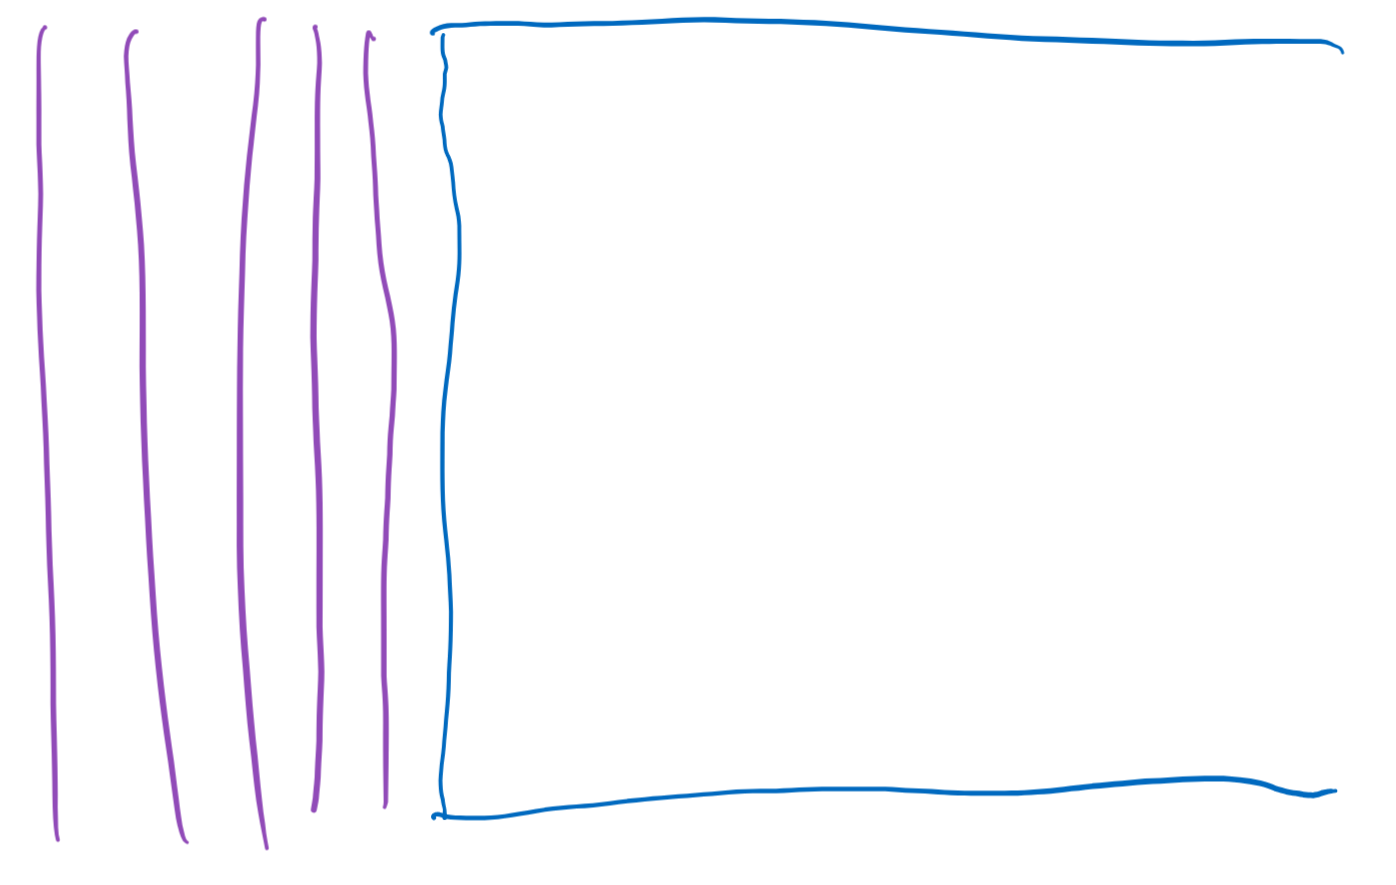
\includegraphics[width=.70\textwidth]{Foliation example.png}
	\label{fig:Foliation example}
\end{figure}


\end{frame}


\subsection{Idea: Relation to gauge theory}

\renewcommand\insertreferences{{\tiny Camille Laurent-Gengoux and Leonid Ryvkin, The holonomy of a singular leaf, \newline \textit{Selecta Mathematica 28}, no.\ 2, 45, 2022.}}

\begin{frame}
\begin{figure}[htbp]
	\centering
		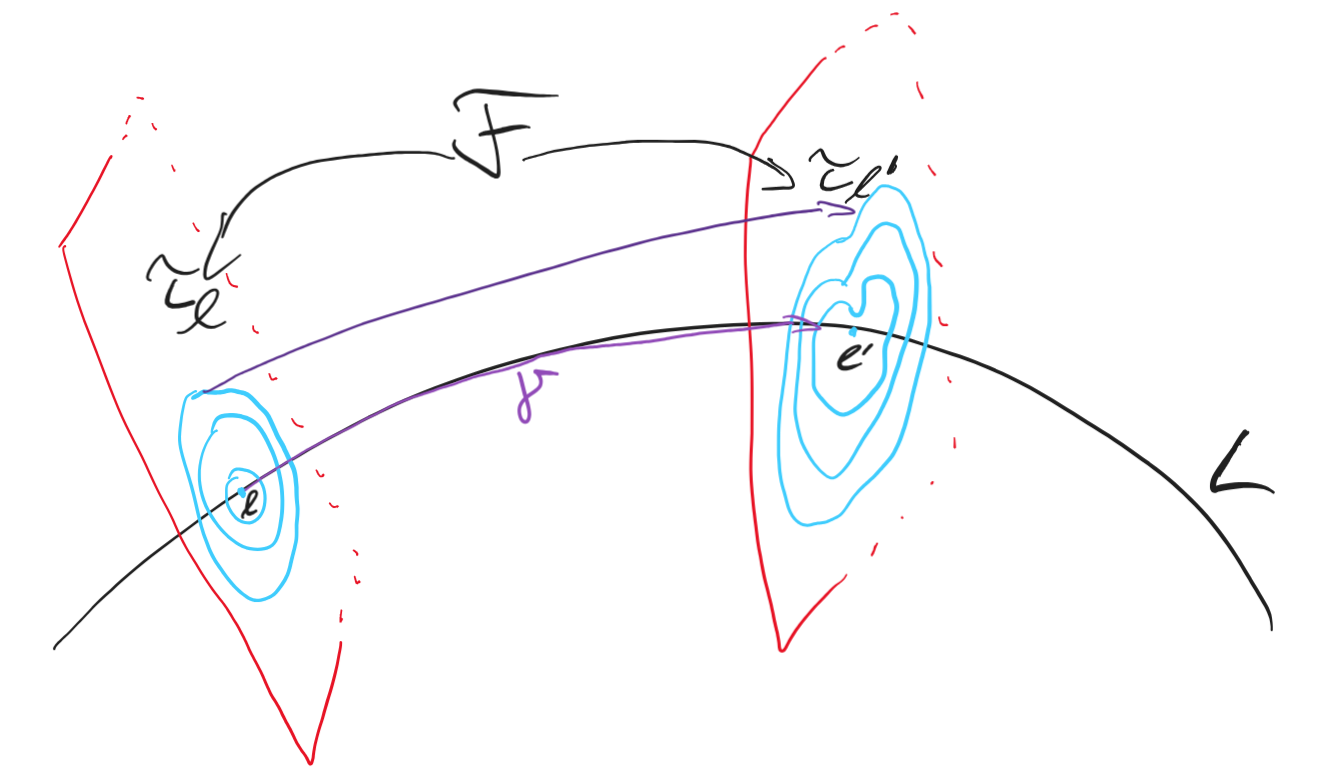
\includegraphics[width=1.00\textwidth]{Foliation connection.png}
	%\caption{$\mathcal{F}$-connections}
	\label{fig:Foliation connection}
\end{figure}

\end{frame}

\begin{frame}
\begin{figure}[htbp]
	\centering
		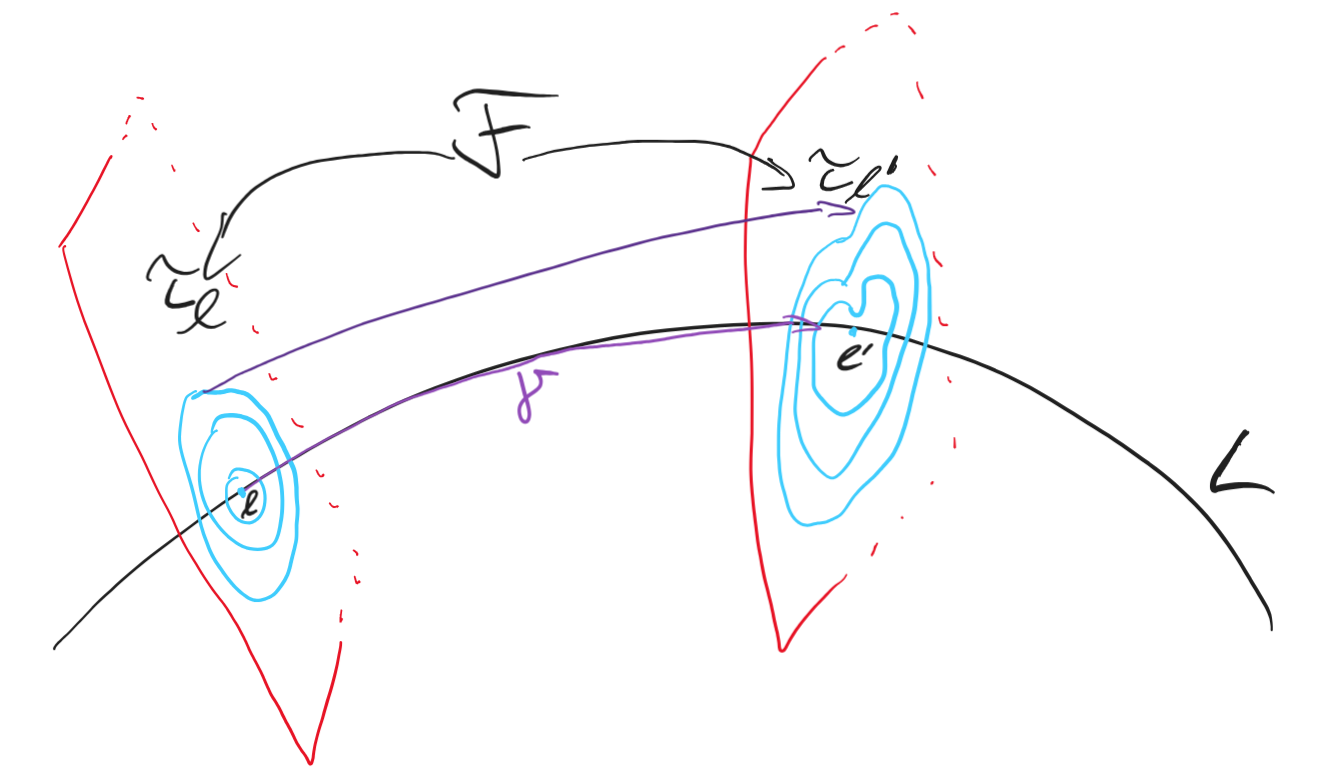
\includegraphics[width=0.50\textwidth]{Foliation connection.png}
	%\caption{$\mathcal{F}$-connections}
	\label{fig:Foliation connection Zwei}
\end{figure}

\begin{theorem}[$\mathcal{F}$-connections]
There is a connection on the normal bundle of a leaf $L$:
\begin{itemize}
	\item Horizontal vector fields are in $\mathcal{F}$.
	\item Parallel transport $\mathup{PT}_\gamma$ has values in $\mathup{Sym}(\tau_l, \tau_{l^\prime})$.
	\item For a contractible loop $\gamma_0$ at $l$: $\mathup{PT}_{\gamma_0}$ values in $\mathup{Inner}(\tau_l)$.
\end{itemize}
\end{theorem}

\end{frame}

\begin{frame}{Example of a transverse foliation $\tau$:}
%\begin{center}
\begin{minipage}[]{0.45\textwidth}
\begin{figure}
\begin{tikzpicture}
\coordinate (O) at (0,0);
\foreach \k in {1,...,4}\pgfmathparse{12*\k} \draw[fill=blue!\pgfmathresult] (O) circle (3.6-0.8*\k) node at (0, 3) {$\mathbb{S}^n$};
\fill (O) circle[radius=2pt];
\end{tikzpicture}
\end{figure}
%\end{center}
\end{minipage}
\hfill
\begin{minipage}[]{0.45\textwidth}
\begin{remark}
\begin{itemize}
	\item $\mathup{Inner}(\tau_l)$ maps each circle to itself
	\item $\mathup{Sym}(\tau_l)$ allows to exchange circles
	\item Both preserve $\tau_l$ and fix the origin
\end{itemize}
\end{remark}
\end{minipage}
\end{frame}

{
\setbeamertemplate{footline}{}

\begin{frame}{Idea}
\begin{figure}[htbp]
	\centering
		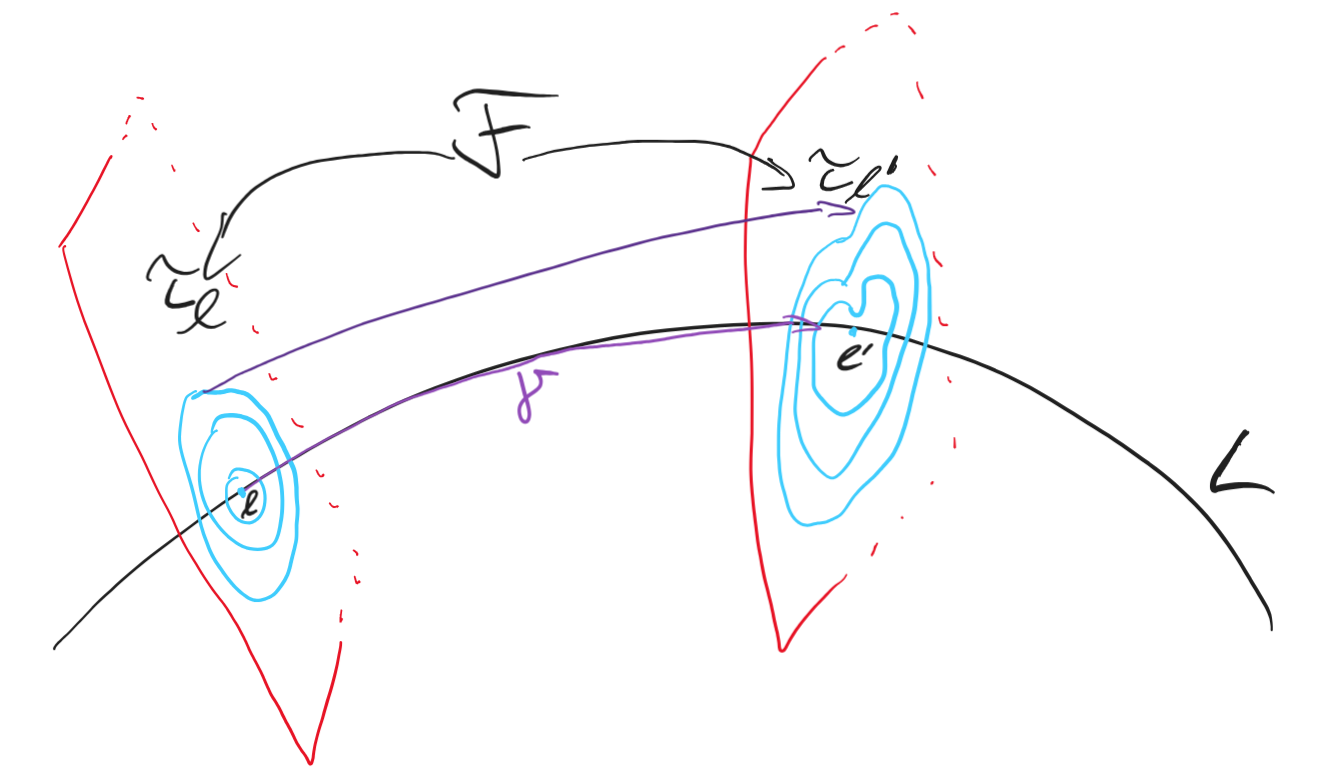
\includegraphics[width=0.5\textwidth]{Foliation connection.png}
	%\caption{$\mathcal{F}$-connections}
	\label{fig:Foliation connection Drei}
\end{figure}

\begin{idea}
Generators of $\mathcal{F}$ given by $\mathcal{F}_{\mathup{projectable}}$:
\bas
\mathbb{H}(X) + \overline{\nu},
\eas
where $X \in \mathfrak{X}(L)$, $\mathbb{H}(X)$ its projectable horizontal lift, $\nu \in \Gamma(\mathrm{inner}(\tau))$ and $\overline{\nu}$ its fundamental vector field.

\end{idea}
\end{frame}

\begin{frame}
\begin{figure}[htbp]
	\centering
		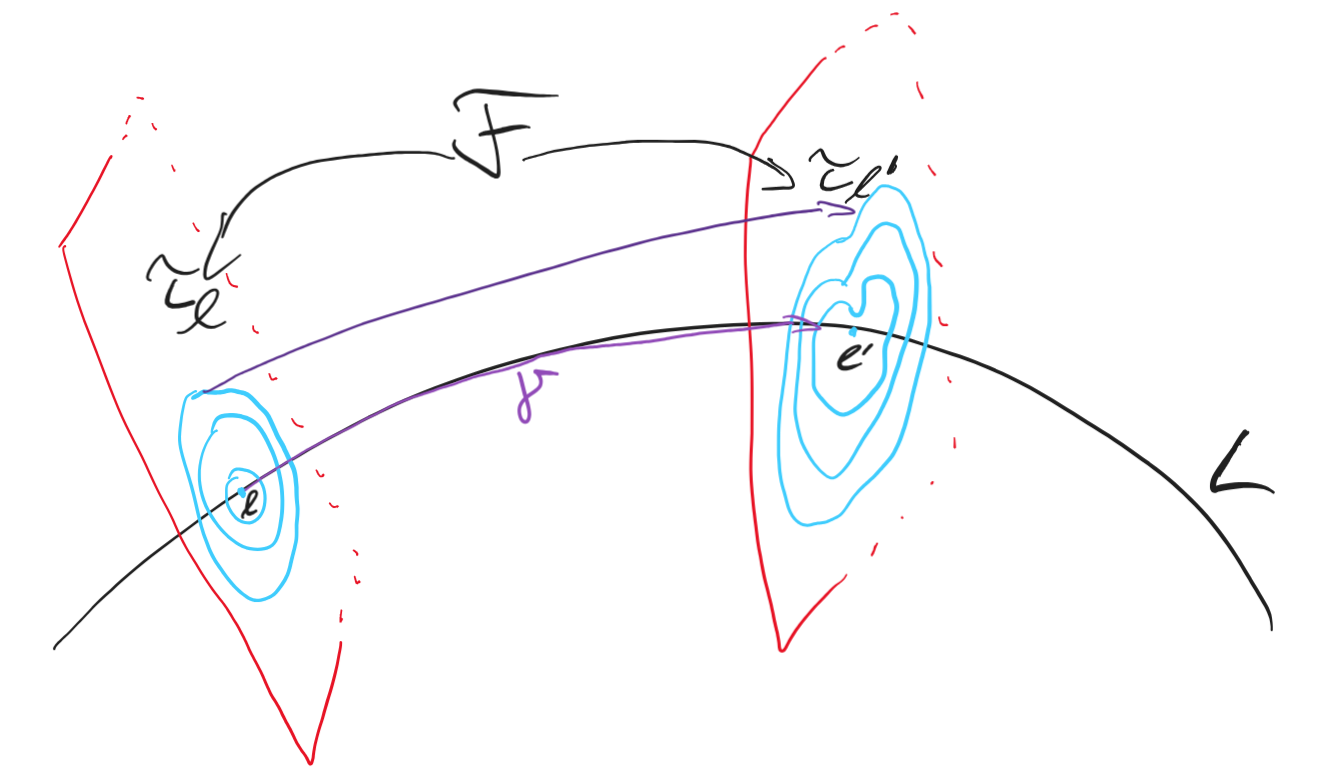
\includegraphics[width=0.5\textwidth]{Foliation connection.png}
	%\caption{$\mathcal{F}$-connections}
	\label{fig:Foliation connection Vier}
\end{figure}
\begin{idea}
Fix $l$ and given $\tau_l$: Reconstruct $\mathcal{F}$.
\bas
\mleft[ \mathbb{H}(X) + \overline{\nu}, \mathbb{H}\mleft({X^\prime}\mright) + \overline{\mu} \mright]
&=
\mathbb{H}\mleft(\mleft[ X, X' \mright]\mright) + 
\overline{\vphantom{d}
\dots
}
\\
&=
\underbrace{\mleft[ \mathbb{H}(X), \mathbb{H}\mleft({X^\prime}\mright) \mright]}_{\rightsquigarrow \text{ curvature}}
\\
&\hspace{1cm}
	+ \underbrace{\mleft[ \mathbb{H}(X), \overline{\mu} \mright]
	- \mleft[ \mathbb{H}\mleft({X^\prime}\mright), \overline{\nu} \mright]}_{\rightsquigarrow \text{ connection}}
	+ \overline{\mleft[ \nu, \mu \mright]}
\eas
\end{idea}
\end{frame}
}

%\section{Curved Yang-Mills gauge theory}





%\section{Foliations and Yang-Mills connections}
\subsection{Reconstructing Foliations}
{
\setbeamertemplate{footline}{}


\begin{frame}
\begin{theorem}[{[C.\ L.-G., S.-R.\ F.]}]
Given a multiplicative Yang-Mills connection on $\mathcal{G}$ and a Yang-Mills connection $\mathbb{H}$ on $\mathcal{T}$, then there is a natural foliation on $\mathcal{T}$ generated by 
\bas
\mathbb{H}(X) + \overline{\nu},
\eas
where $X \in \mathfrak{X}(L)$ and $\nu \in \Gamma(\mathcal{g})$.
\end{theorem}
\pause
\begin{proof}
We have
\bas
\mleft[ \mathbb{H}(X), \overline{\nu} \mright]
&=
\overline{ \nabla_X \nu },
\\
\mleft[ \mathbb{H}(X), \mathbb{H}(X^\prime) \mright]
&=
\mathbb{H}\mleft(\mleft[ X, X^\prime \mright]\mright)
	+ \overline{\zeta\mleft(X, X^\prime\mright)},
\eas
where $\zeta \in \Omega^2(L; \mathcal{g})$.	
\end{proof}
\end{frame}

\begin{frame}
\begin{idea}[Leaf $L$ simply connected]
Fix a point $l \in L$ with transverse model $\mleft(\mathbb{R}^d, \tau_l\mright)$:
\begin{enumerate}
	\item $G = \mathrm{Inn}(\tau_l)$
	\pause
	\item $P$ a principal $G$-bundle, equipped with an ordinary connection
	%\pause
	%\item 
	\pause
	\item $\mathcal{G} \coloneqq (P \times G) \Big/ G$, the \textbf{inner group bundle}
	\pause
	\item $\mathcal{T} \coloneqq \mleft(P \times \mathbb{R}^d\mright) \Big/ G$, the \textbf{normal bundle}
\end{enumerate}
\end{idea}

\pause

\begin{remark}
\begin{itemize}
	\item Think of the induced connection on $\mathcal{T}$ as the $\mathcal{F}$-connection.
	\item $\mathcal{G}$ acts on $\mathcal{T}$ (canonically from the left).
\end{itemize}
\end{remark}

\end{frame}

\begin{frame}
\begin{proposition}[{[C.\ L.-G., S.-R.\ F.]}]
The associated connection on $\mathcal{G}$ is a multiplicative Yang-Mills connection and the one on $\mathcal{T}$ is a corresponding Yang-Mills connection.
\end{proposition}

\begin{remark}
Thus, we have a singular foliation on $\mathcal{T}$, which, by construction, admits $L$ as a leaf and $\tau_l$ as transverse data.
\end{remark}
\end{frame}

{
\setbeamertemplate{footline}{}

\subsection{Independency of choice of connection}


\begin{frame}
\begin{proposition}[{[C.\ L.-G., S.-R.\ F.]}]
The reconstructed foliation is independent of the choice of connection on $P$.
\end{proposition}
\pause
\begin{center}
\begin{tikzcd}[ampersand replacement=\&]
	\Gamma(\mathrm{Ad}(P)) \arrow[hook]{dr} \arrow{rrrr}{\nu \mapsto \overline{\nu}} 
        \&\&\&\& 
        \tau \arrow[hook]{dl}
        \\
        \& 
        \Gamma(\mathrm{At}(P)) \arrow[two heads]{dr} \arrow{rr}{\xi \mapsto \overline{\xi}} 
        \&\&
        \mathcal{F}_{\mathup{projectable}} \arrow[two heads]{dl}
        \&
        \\
        \&\& \arrow[bend left]{ul}{A} \mathfrak{X}(L) \arrow[bend right, swap]{ur}{\mathbb{H}} \&\&
	\end{tikzcd}
\end{center}
\end{frame}

\subsection{Summary}

\begin{frame}{Summary}
\begin{remark}[{[C.\ L.-G., S.-R.\ F.]}]
In the simply connected case, the following are equivalent:
\begin{itemize}
	\item Singular foliations with leaf $L$ and transverse model $\mleft(\mathbb{R}^d, \tau_l\mright)$
	\item Principal $\mathrm{Inner}(\tau_l)$-bundles over $L$
\end{itemize}
\end{remark}

\end{frame}

\begin{frame}
\begin{remark}[Classification of curved Yang-Mills gauge theories]
If $\mathcal{G}$ acts faithfully on $\mathcal{T}$, preserving $L$, then a curved Yang-Mills gauge theory can be flattened if and only if $P$ is flat.
\end{remark}

\begin{table}[h!]
		\begin{tabularx}{\textwidth}{X X}
			\rowcolor{gray}
			Curved YM Gauge Theory & Singular Foliations $\mathcal{F}$ \\
			Multiplicative Yang-Mills connection & $\mathcal{F}$-connection \\
			\rowcolor{Gray}
			Flat gauge theory & Flat singular foliation \\
			Field redefinition of connection on $\mathcal{G}$ & Different choice of $\mathcal{F}$-connection
		\end{tabularx}
\end{table}
\end{frame}

}

%\section{Future Prospects}
%{
%\setbeamertemplate{footline}{}
%\begin{frame}
%
%\begin{remark}[Future prospects]
%\begin{itemize}
	%\item Further applications of curved gauge theories (existence of Cartan connections,...)
	%\item Total space and Atiyah bundles of groupoid-based principal bundles
	%\item Field redefinitions as natural symmetry in associated applications
%\end{itemize}
%\end{remark}
%
%\end{frame}
%}
\thispagestyle{empty}
\topmargin -3.46 cm
\vspace*{\fill}
\begin{center}
\huge \textbf{Thank you!}
\end{center}
\vspace*{\fill}

\end{document}

